\hypersection{ch3914}{サンプリング分布(sampling distributions)}
\index{さんぷりんぐぶんぷ@サンプリング分布}\index{らんすうぶんぷ@乱数分布!さんぷりんぐぶんぷ@サンプリング分布}

サンプリング分布(sampling distributions)とは、標本から分布の特徴がわかっている場合に、その特徴を指定することにより、望みの分布を作り出す分布のことだ。

\hypersubsection{ch391401}{離散分布(std::discrete\texttt{\_}distribution\texttt{<}IntType\texttt{>})}
\index{りさんぶんぷ@離散分布}\index{らんすうぶんぷ@乱数分布!りさんぶんぷ@離散分布}

\hypersubsubsection{ch39140101}{簡単な説明}

離散分布(discrete distribution)は整数型の乱数\(i\), \(0 \leq i < n\)を返す分布だ。例えば\(n = 10\)ならば、\(0,1,2,3,4,5,6,7,8,9\)の10個のうちのいずれかの整数値を乱数として返す。この際、乱数値として取りうる整数値1つ1つに、確率を設定できる。確率は\(p_0, \cdots, p_{n-1}\)で設定し、\(p_0\)が\(0\)の確率, \(p_1\)が\(1\)の確率\ldots{}\(p_{n-1}\)が\(n\)の確率となる。それぞれの乱数\(i\)は確率\(\frac{p_i}{S}\)で出現する。このとき\(S\)とはすべての確率の合計、つまり\(S = p_0 + \cdots + p_{n-1}\)となる。確率\(p_i\)は\texttt{double}型で与える。

たとえば、\texttt{\{1.0, 1.0, 1.0\}}\,という確率群を渡した場合、離散分布は\(0, 1, 2\)のいずれかの乱数をそれぞれ\(\frac{1.0}{3.0}\)の確率で返す。

もし、\texttt{\{1.0, 2.0, 3.0\}}という確率群を渡した場合、離散分布は\(0, 1, 2\)のいずれかの乱数を返す。その時の確率は、\(1\)が\(\frac{1}{6}\)、\(2\)が\(\frac{1}{3}\)、\(3\)が\(\frac{1}{2}\)だ。

例えば公平な6面ダイスを作りたい場合、\texttt{\{1.0, 1.0, 1.0, 1.0, 1.0, 1.0\}}\,を指定すると\(0 \leq i \leq 5\)までの6個の乱数\(i\)がそれぞれ\(\frac{1}{6}\)の確率で生成される。この結果に\texttt{+1}すると\(1 \leq i \leq 6\)の乱数を得ることができる。

6の目だけ2倍高い確率で出るイカサマ6面ダイスを作りたい場合、\texttt{\{1.0, 1.0, 1.0, 1.0, 1.0, 2.0\}}\,を指定すると、0から4までの5つの目は\(\frac{1}{7}\)の確率で出現し、5だけは\(\frac{2}{7}\)の確率で出る乱数を作ることができる。

\(S\)はすべての確率の合計で、それぞれの値は\(\frac{p_i}{S}\)の確率で出る。なので、以下はすべて分布だ。

\begin{lstlisting}[style=terminal]
{1.0, 1.0, 1.0, 1.0, 1.0, 2.0}
{0.1, 0.1, 0.1, 0.1, 0.1, 0.2}
{2.0, 2.0, 2.0, 2.0, 2.0, 4.0}
\end{lstlisting}

\hypersubsubsection{ch39140102}{数学的な説明}

\texttt{std::discrete\_distribution<IntType>}\,\index{discrete\_distribution@\texttt{discrete\_distribution}}は整数型の乱数\(i\), \(0 \leq i < n\)を以下の離散確率関数に従って分布する。
\[
P(i \,|\, p_0, \cdots, p_{n-1}) = p_i \text{ .}
\]

別に指定のない場合、分布パラメーターは\(p_k = {w_k / S}\) for \(k = 0, \cdots, n - 1\)として計算され、このとき値\(w_k\)は、一般に\emph{ウエイト(weight)}と呼ばれていて、値は非負数、非NaN、非無限でなければならない。さらに、以下の関係が成り立たねばならない。\(0 < S = w_0 + \dotsb + w_{n - 1}\)。

\hypersubsubsection{ch39140103}{変数の宣言}

\texttt{std::discrete\_distribution}の変数を宣言するには3つの方法がある。いずれも\texttt{double}型の値を\texttt{n}個渡すための方法だ。

\vskip 1.0zw
\noindent
\(\bullet\) \textsf{イテレーターのペア}

\noindent
\textsf{変数の宣言:}

\begin{lstlisting}[style=grammar]
std::discrete_distribution<IntType> d( firstW, lastW ) ;
\end{lstlisting}

\texttt{IntType}は整数型でデフォルトは\texttt{int}、\texttt{[firstW, lastW)}はイテレーターのペアで、\texttt{double}型に変換可能な値を参照している。

\vskip 1.0zw
\noindent
\textsf{利用例:}

\begin{lstlisting}[language={C++}]
int main()
{
    std::array ps = {1.0, 2.0, 3.0} ;
    std::discrete_distribution d( std::begin(ps), std::end(ps) );

    std::mt19937 e ;
    d(e)
}
\end{lstlisting}

\vskip 1.0zw
\noindent
\(\bullet\) \textsf{初期化リスト}

\noindent
\textsf{利用例:}

\begin{lstlisting}[style=grammar]
std::discrete_distribution<IntType> d( {...} ) ;
std::discrete_distribution<IntType> d = {...} ;
\end{lstlisting}

\texttt{...}には\texttt{double}型の浮動小数点数を指定する

\vskip 1.0zw
\noindent
\textsf{利用例:}

\begin{lstlisting}[language={C++}]
int main()
{
    std::discrete_distribution d( { 1.0, 2.0, 3.0 } );
    // もしくは
    // ... d = { 1.0, 2.0, 3.0 } ;

    std::mt19937 e ;
    d(e)
}
\end{lstlisting}

\vskip 1.0zw
\noindent
\(\bullet\) \textsf{個数、デルタ、関数}

このコンストラクターは以下のように宣言されている。

\begin{lstlisting}[style=grammar]
template<class UnaryOperation>
discrete_distribution(
    size_t nw,
    double xmin, double xmax,
    UnaryOperation fw
);
\end{lstlisting}

\texttt{UnaryOperation}は1つの実引数を取る関数オブジェクトで戻り値の型は\texttt{double}型に変換できること。さらに、\texttt{double}型は\texttt{UnaryOperation}の引数に変換可能なこと。もし\(nw = 0\)の場合は、\(n = 1\)とする。それ以外の場合、\(n = {\tt nw}\)とする。このとき、\(0 < \delta = ({\tt xmax} - {\tt xmin}) / n\)となる関係が満たされなければならない。

もし\(nw = 0\)ならば\(w_0 = 1\)。それ以外の場合、\(k = 0, \cdots, n - 1\)に対して、\(w_k = {\tt fw}({\tt xmin} + k \cdot \delta + \delta / 2)\)とする。\texttt{fw}は\texttt{n}回を超えて呼ばれることはない。

\begin{lstlisting}[language={C++}]
int main()
{
    std::discrete_distribution d( 5, 0.0, 1.0, [](auto x){
        std::cout << x << '\n' ;
        if ( x < 0.3 )
            x = 0.3 ;
        if ( x > 0.8 )
            x = 0.8 ;
        return x ;
    } );
}
\end{lstlisting}

\ifTombow\pagebreak\fi
この\texttt{d}は、
\begin{lstlisting}[style=grammar]
std::discrete_distribution d = {0.3, 0.3, 0.5, 0.7, 0.8 } ;
\end{lstlisting}
と初期化されたものと同じように初期化される。

\hypersubsubsection{ch39140104}{初期化パラメーターの確認}

\texttt{std::discrete\_distribution}の内部状態はメンバー関数\texttt{probabilities}で取得できる。戻り値の型は\texttt{std::vector<double>}で、指定した確率群が要素になっている。

\begin{lstlisting}[language={C++}]
int main()
{
    std::discrete_distribution d = { 1.0, 2.0, 3.0 } ;
    auto v = d.probabilities() ;
    // vは{1.0, 2.0, 3.0}
}
\end{lstlisting}

\hypersubsubsection{ch39140105}{応用例}

以下は6の目が2倍の確率で出るイカサマ6面ダイスの実装だ。

\begin{lstlisting}[language={C++}]
template < typename Engine >
int roll_dice( Engine & e )
{
    std::discrete_distribution d = { 1.0, 1.0, 1.0, 1.0, 1.0, 2.0 } ;
    return d(e) + 1 ;
}
\end{lstlisting}

\hypersubsection{ch391402}{区分定数分布(std::piecewise\texttt{\_}constant\texttt{\_}distribution\texttt{<}RealType\texttt{>})}
\index{くぶんていすうぶんぷ@区分定数分布}\index{らんすうぶんぷ@乱数分布!くぶんていすうぶんぷ@区分定数分布}

\hypersubsubsection{ch39140201}{簡単な説明}

区分定数分布(piecewise constant distribution)とは、区分と、区分ごとの確率を指定し、いずれかの区分の範囲の値に一様分布させる分布だ。ここでいう確率は、密度、あるいはウエイトともいう。

1つの区分は\texttt{double}型の値2つ\(b_i, b_{i+1}\)で与える。このとき区分の乱数\(x\)の範囲は\([b_i, b_{i+1})\)、もしくは\(b_i \leq x < b_{i+1}\)だ。\(n\)個の値を指定すると、\(n-1\)個の区分を指定したことになる。

例えば\,\texttt{\{0.0, 1.0\}}\,という2つの\texttt{double}型の値を使って1つの区分を与えた場合、これは\(0.0 \leq x < 1.0\)という値の範囲の区分である。\texttt{\{0.0, 1.0, 2.0\}}\,という3つの\texttt{double}型の値は2つの区分になり、それぞれ\(0.0 \leq x < 1.0\), \(1.0 \leq x < 2.0\)になる。

一般に、\(n\)個の\texttt{double}型の値\(b_0, \cdots, b_n\)で\(n-1\)個の区分を表現する。このとき、\(b_i < b_{i+1}\)が\(i = 0, \cdots, n-1\)までの\(i\)について成り立たなければならない。つまり区分を指定する\texttt{double}型の値は、後続の値より小さくなければならないということだ。

以下は正しい区分の指定だ。

\begin{lstlisting}[style=terminal]
{1.0, 2.0, 100.0, 999.999}
{-1.0, 1.0, 2.0}
{-5.0, -4.0, -3.1}
\end{lstlisting}

以下は正しくない区分の指定だ。

\begin{lstlisting}[style=terminal]
{1.0, 0.0}
\end{lstlisting}

これは\(b_0 > b_1\)なので正しくない。

それぞれの区分\([b_i, b_{i+1})\)に対して確率\(p_i\)を\texttt{double}型で指定する。\(n\)個の\(b_i\)によって\(n-1\)個の区分を指定し、それぞれに対して1つずつ確率を設定するので、確率の数は\(n-1\)個だ。

例えば\,\texttt{\{0.0, 1.0\}}\,という1つの区分と\,\texttt{\{1.0\}}\,という1つの確率を与えた場合、\(0.0 \leq x < 1.0\)の範囲の乱数\(x\)が生成される。

\texttt{\{0.0, 1.0, 10.0\}}\,という2つの区分と、\texttt{\{1.0, 2.0\}}\,という2つの確率を与えた場合、\(\frac{1}{3}\)の確率で\(0.0 \leq x < 1.0\)の範囲に一様分布した乱数になり、\(\frac{2}{3}\)の確率で\(1.0 \leq x < 10.0\)の範囲に一様分布した乱数になる。

\hypersubsubsection{ch39140202}{数学的な説明}

\texttt{std::piecewise\_constant\_distribution<RealType>}\,\index{piecewise\_constant\_distribution@\texttt{piecewise\_constant\_distribution}}は浮動小数点数型の乱数\(x\), \(b_0 \leq x < b_n\)を以下の確率密度関数に従って、それぞれの部分区間(subinterval)\([b_i, b_{i+1})\)の間で一様に分布させる。
\[
p(x \,|\, b_0, \cdots, b_n, \; \rho_0, \cdots, \rho_{n-1}) = \rho_i
   \text{ , for $b_i \le x < b_{i+1}$.} 
\]

この分布の区間境界(interval boundaries)ともいう\(n+1\)分布パラメーター\(b_i\)はすべての\(i = 0, \cdots, n - 1\)に対して関係\(b_i < b_{i + 1}\)を満たさねばならない。別途指定なき場合、残りの\(n\)分布パラメーターは以下のように計算される。
\[
\rho_k = \frac{w_k}{S \cdot (b_{k+1}-b_k)} \text{ for } k = 0, \cdots, n - 1 \text{ ,} 
\]

一般にウエイト(weight)と呼ばれている値\(w_k\)は、非負数、非NaN、非無限でなければならない。さらに、以下の関係を満たさなければならない。

\(0 < S = w_0 + \dotsb + w_{n-1}\)

\hypersubsubsection{ch39140203}{変数の宣言}

\texttt{std::piecewise\_constant\_distribution}では、\texttt{double}型の値の集合を2つ渡す必要がある。1つは区間を指定するための\(N\)個の\texttt{double}型に変換可能な値で、もう1つは区間ごとの確率を指定するための\(N-1\)個の\texttt{double}型に変換可能な値だ。

\vskip 1.0zw
\noindent
\(\bullet\) \textsf{イテレーターによる指定}

イテレーターで区間と確率を指定するコンストラクターは以下のとおり。

\begin{lstlisting}[style=grammar]
template<class InputIteratorB, class InputIteratorW>
piecewise_constant_distribution(
    InputIteratorB firstB, InputIteratorB lastB,
    InputIteratorW firstW
);
\end{lstlisting}

\texttt{[firstB, lastB)}は区間を指定するための\(N\)個の値を参照する入力イテレーターのペアだ。\texttt{firstW}はそれぞれの区間の確率を指定する\(N-1\)個の値を参照する入力イテレーターの先頭だ。\texttt{lastW}がないのは、確率の個数は\(N-1\)個であるとわかっているからだ。

もし\texttt{[firstB, lastB)}のサイズが1以下の場合、区間は\texttt{[0.0, 1.0)}になり、確率は\(\frac{1}{1}\)になる。

\vskip 1.0zw
\noindent
\textsf{利用例:}

\begin{lstlisting}[language={C++}]
int main()
{
    std::array bs = {-1.0, 1.0, 2.0 } ;
    std::array ps = { 1.0, 5.0 } ;
    std::piecewise_constant_distribution d( std::begin(bs), std::end(bs), std::begin(ps) ) ;

    std::mt19937 e ;
    d(e) ;
}
\end{lstlisting}

\texttt{bs}は区間を指定する値の集合、\texttt{ps}は区間ごとの確率だ。

区間は\texttt{[-1.0, 1.0)}と\texttt{[1.0, 2.0)}の2つ。確率はそれぞれ\(\frac{1}{6}\)、\(\frac{5}{6}\)だ。

区間を表現する値が足りない場合は以下のとおり。

\begin{lstlisting}[language={C++}]
int main()
{
    // 区間を指定すべき値が足りない
    std::array bs = { 1.0 } ;
    std::array ps = { 1.0, 5.0 } ;
    // 引数は無視される。
    // 区間は[0.0, 1.0), 確率は100%
    std::piecewise_constant_distribution d( std::begin(bs), std::end(bs), std::begin(ps) ) ;
}
\end{lstlisting}

\vskip 1.0zw
\noindent
\(\bullet\) \textsf{初期化リストと関数オブジェクトによる指定}

初期化リストと関数を指定するコンストラクターは以下のとおり。

\ifTombow\pagebreak\fi
\begin{lstlisting}[style=grammar]
template<class UnaryOperation>
piecewise_constant_distribution(
    initializer_list<RealType> bl,
    UnaryOperation fw
);
\end{lstlisting}

イテレーターのペアと同じく、区間は\texttt{[bl.begin(), bl.end())}で指定する。

確率は\(k = 0, \cdots, n - 1\)について、\(w_k = {\tt fw}\bigl(\bigl(b_{k+1} + b_k\bigr) / 2\bigr)\)とする。

\texttt{bl.size()}が1以下の場合、区間は\texttt{[0.0, 1.0)}になり、確率は\(\frac{1}{1}\)になる。

\vskip 1.0zw
\noindent
\textsf{利用例:}

\begin{lstlisting}[language={C++}]
int main()
{
    std::piecewise_constant_distribution d(
        {1.0, 2.0, 3.0, 4.0, 5.0},
        []( auto x )
        { return x ; }
    ) ;
}
\end{lstlisting}

この場合、区間は\texttt{[1.0, 2.0)}, \texttt{[2.0, 3.0)}, \texttt{[3.0, 4.0)}, \texttt{[4.0, 5.0)}の4個になり、確率は\,\texttt{\{1.5, 2.5, 3.5, 4.5\}}\,となる。

\vskip 1.0zw
\noindent
\(\bullet\) \textsf{区間数、最小、最大、関数オブジェクトによる指定}

\noindent
\textsf{コンストラクターの宣言:}

\begin{lstlisting}[style=grammar]
template<class UnaryOperation>
piecewise_constant_distribution(
    size_t nw,
    RealType xmin, RealType xmax,
    UnaryOperation fw
);
\end{lstlisting}

\texttt{nw}は区間数、\texttt{xmin}は最小値、\texttt{xmax}は最大値、\texttt{fw}は関数オブジェクトで、\texttt{double}型から変換できる型の実引数を取り、\texttt{double}型に変換可能な戻り値を返す。

\(nw = 0\)の場合、区間の個数\(n\)は\(1\)になる。それ以外の場合、\(n = nw\)となる。このとき関係、\(0 < \delta = ({\tt xmax} - {\tt xmin}) / n\)が成り立たなければならない。
\begin{align*}
  &\text{Let}\quad b_k = {\tt xmin} + k \cdot \delta  \quad\text{for  $k = 0, \cdots, n$,}\\
  &\text{and}\quad w_k = {\tt fw}(b_k + \delta / 2)   \quad\text{for} .
\end{align*}

\(k = 0, \cdots, n - 1\)において、区間は\(b_k = {\tt xmin} + k \cdot \delta \text{for $ k = 0, \cdots, n$}\)とし、確率は\(w_k = {\tt fw}(b_k + \delta / 2)\)とする。

\vskip 1.0zw
\noindent
\textsf{利用例:}

\begin{lstlisting}[language={C++}]
int main()
{
    std::piecewise_constant_distribution d( 5, 1.0, 5.0,
        []( auto x ) { return x ; } ) ;
}
\end{lstlisting}

この場合、区間の集合は\,\texttt{\{1.0, 1.8, 2.6, 3.4, 4.2, 5.0\}}\,となり、確率は\,\texttt{\{1.4, 2.2, 3.0, 3.8, 4.6\}}\,となる。

\hypersubsubsection{ch39140204}{内部状態の取得}

\texttt{std::piecewise\_constant\_distribution}の内部状態は、メンバー関数\texttt{intervals}と\texttt{densities}で得ることができる。

\begin{lstlisting}[style=grammar]
template<class RealType = double>
class piecewise_constant_distribution {
public :
    vector<result_type> intervals() const;
    vector<result_type> densities() const;
} ;
\end{lstlisting}

\texttt{intervals}は区間、\texttt{densities}は確率を返す。

\begin{lstlisting}[language={C++}]
int main()
{
    auto bs = { 1.0, 2.0, 3.0 } ;
    auto ps = { 1.0, 2.0 } ;
    std::piecewise_constant_distribution d( std::begin(bs), std::end(bs), std::begin(ps) ) ;

    // {1.0, 2.0, 3.0}
    auto intervals = d.intervals() ;
    // {0.333333, 0.666667}
    auto densities = d.densities() ;
}
\end{lstlisting}

\texttt{densities()}の結果が正規化されているのは、ユーザーが指定した確率は\(w_k\)だが、ここで返すのは\(p_k\)だからだ。

\hypersubsection{ch391403}{区分線形分布(std::piecewise\texttt{\_}linear\texttt{\_}distribution\texttt{<}RealType\texttt{>})}
\index{くぶんせんけいぶんぷ@区分線形分布}\index{らんすうぶんぷ@乱数分布!くぶんせんけいぶんぷ@区分線形分布}

\hypersubsubsection{ch39140301}{簡単な説明}

区分線形分布(piecewise linear distribution)は区分定数分布と同じく、区間と確率(またの名を密度、ウエイト)を指定する。

区間の指定は区分定数分布と同じだ。内部境界の集合で指定する。例えば\,\texttt{\{1.0, 2.0, 3.0\}}\,は2つの区間\texttt{[1.0, 2.0)}と\texttt{[2.0, 3.0)}を指定する。

区分線形分布における確率は、区間に対してではなく、内部境界に対して指定する。指定した全区間における値の出現確率は、内部境界から内部境界に向かって指定した確率の差の方向に線形に増加、もしくは減少する。

例えば区分\,\texttt{\{0.0, 1.0\}}\,と確率\,\texttt{\{1.0, 2.0\}}\,を指定した場合、これは1つの区間\texttt{[0.0, 1.0)}について、内部境界\texttt{0.0}の確率は\(\frac{1}{3}\)、内部境界\texttt{1.0}の確率は\(\frac{2}{3}\)とし、\(0.0 \leq x < 1.0\)の範囲の乱数\texttt{x}を生成する。内部境界区間の範囲に注意。\texttt{1.0}未満なので、\texttt{1.0}は出ない。

そして、区間の間の値は、区間を区切る2つの内部境界の確率の差によって、線形に増加、もしくは減少する。例えば値\texttt{0.25}が出る確率は\(\frac{1.25}{3}\)、\texttt{0.5}が出る確率は\(\frac{1.5}{3}\)、値\texttt{1.75}が出る確率は\(\frac{1.75}{3}\)だ。

区分\,\texttt{\{0.0, 1.0, 2.0\}}\,と確率\,\texttt{\{1.0, 2.0, 1.0\}}\,の場合、2つの区間\texttt{[0.0, 1.0)}と\texttt{[1.0, 2.0)}の範囲について、\texttt{0.0}から\texttt{1.0}に向かう区間についての確率は\(\frac{1}{4}\)から\(\frac{1}{2}\)に増加し、\texttt{1.0}から\texttt{2.0}に向かう区間についての確率は\(\frac{1}{2}\)から\(\frac{1}{4}\)に減少する。

結果として、乱数値の分布をグラフに描画すると、\texttt{1.0}が最も出やすく、その前後±1.0の範囲で徐々に減少していく山のようなグラフになる。

\begin{figure}[htbp]
  \centering
  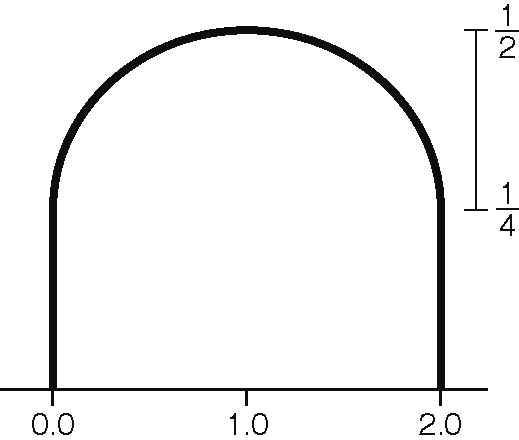
\includegraphics[scale=1.0]{fig/fig39-01.eps}
  \label{fig:37-01}
\end{figure}

\hypersubsubsection{ch39140302}{数学的な説明}

\texttt{std::piecewise\_linear\_distribution<RealType>}\,\index{piecewise\_linear\_distribution@\texttt{piecewise\_linear\_distribution}}は乱数\(x\), \(b_0 \leq x < b_n\)を以下の確率密度関数に従って分布する。
\[
p(x \,|\, b_0, \cdots, b_n, \; \rho_0, \cdots, \rho_n)
     = \rho_{i}   \cdot {\frac{b_{i+1} - x}{b_{i+1} - b_i}}
     + \rho_{i+1} \cdot {\frac{x - b_i}{b_{i+1} - b_i}}
     \text{ , for $b_i \le x < b_{i+1}$.} 
\]

一般に\emph{内部境界}とも呼ばれる\(n + 1\)分布パラメーター\(b_i\)は\(i = 0, \cdots, n - 1\)において関係\(b_i < b_{i+1}\) for \(i = 0, \cdots, n - 1\)を満たさねばならない。別記する場合を除いて、残りの\(n + 1\)パラメーターは\(k = 0, \cdots, n\)において\(\rho_k = {w_k / S}\)と計算される。このとき\(w_k\)は一般に境界におけるウエイト(weight at boundaries)と呼ばれ、非負数、非NaN、非無限でなければならない。さらに、以下の関係が成り立たねばならない。
\[
0 < S = \frac{1}{2} \cdot \sum_{k=0}^{n-1} (w_k + w_{k+1}) \cdot (b_{k+1} - b_k) \text{ .}
\]

\hypersubsubsection{ch39140303}{変数の宣言}

\texttt{piecewise\_linear\_distribution}は区間と確率を指定するために\texttt{n}個の\texttt{double}型に変換可能な値を指定する必要がある。

\vskip 1.0zw
\noindent
\(\bullet\) \textsf{イテレーターによる指定}

\begin{lstlisting}[style=grammar]
template<class InputIteratorB, class InputIteratorW>
piecewise_linear_distribution(
    InputIteratorB firstB, InputIteratorB lastB,
    InputIteratorW firstW );
\end{lstlisting}

\texttt{[firstB, lastB)}は区間、\texttt{firstW}から区間数までのイテレーターが確率。

\texttt{firstB == lastB}もしくは\texttt{++firstB == lastB}の場合、つまり内部境界が1個以下で、空の場合、区間数は1つで\texttt{[0.0, 1.0)}の範囲、確率は\,\texttt{\{0.0, 1.0\}}\,となる。

\vskip 1.0zw
\noindent
\textsf{使い方:}

\begin{lstlisting}[language={C++}]
int main()
{
    auto bs = { 0.0, 1.0, 2.0 } ;
    auto ps = { 1.0, 2.0, 1.0 } ;
    std::piecewise_linear_distribution d( std::begin(bs), std::end(bs), std::begin(ps) ) ;

    std::mt19937 e ;
    d(e) ;
}
\end{lstlisting}

空の場合。

\begin{lstlisting}[language={C++}]
int main()
{
    auto bs = { 0.0 } ;
    auto ps = { 0.0 } ;
    std::piecewise_linear_distribution d( std::begin(bs), std::end(bs), std::begin(ps) ) ;
}
\end{lstlisting}

これは以下のコードと同じだ。

\ifTombow\pagebreak\fi
\begin{lstlisting}[language={C++}]
int main()
{
    auto bs = { 0.0, 1.0 } ;
    auto ps = { 0.0, 1.0 } ;
    std::piecewise_linear_distribution d( std::begin(bs), std::end(bs), std::begin(ps) ) ;
}
\end{lstlisting}

\vskip 1.0zw
\noindent
\(\bullet\) \textsf{初期化リストと関数オブジェクトによる指定}

\begin{lstlisting}[style=grammar]
template<class UnaryOperation>
piecewise_linear_distribution(
    initializer_list<RealType> bl,
    UnaryOperation fw
);
\end{lstlisting}

区間を指定する内部境界は\texttt{[bl.begin(), bl.end())}、内部境界\(b_k\)に対する確率\(w_k\)は\(k = 0, \cdots, n\)について、\(w_k = {\tt fw}(b_k)\)とする。

内部境界が1個以下の場合はイテレーターの場合と同じ。

\vskip 1.0zw
\noindent
\textsf{使い方:}

\begin{lstlisting}[language={C++}]
int main()
{
    std::piecewise_linear_distribution d(
        {0.0, 1.0, 2.0},
        [](auto x){ return x ; }
    ) ;
}
\end{lstlisting}

これは以下のコード同じだ。

\begin{lstlisting}[language={C++}]
int main()
{
    auto bs = { 0.0, 1.0, 2.0 } ;
    auto ps = { 0.0, 1.0, 2.0 } ;
    std::piecewise_linear_distribution d( std::begin(bs), std::end(bs), std::begin(ps) ) ;
}
\end{lstlisting}

\ifTombow\pagebreak\else{\vskip 1.0zw}\fi
\noindent
\(\bullet\) \textsf{個数、最小値、最大値、関数オブジェクトによる指定}

\begin{lstlisting}[style=grammar]
template<class UnaryOperation>
piecewise_linear_distribution(
    size_t nw,
    RealType xmin, RealType xmax,
    UnaryOperation fw
);
\end{lstlisting}

\texttt{nw}が個数、\texttt{xmin}が最小値、\texttt{xmax}が最大値、\texttt{fw}が関数オブジェクト。

関数オブジェクト\texttt{fw}は\texttt{double}型から変換できる実引数を1つだけ取り、戻り値の型は\texttt{double}型に変換できること。

\({\tt nw} = 0\)ならば空であり、イテレーターの場合と同じ。

関係\(0 < \delta = ({\tt xmax} - {\tt xmin}) / n\)が成り立つこと。

内部境界\(b_k\)は\(k = 0, \cdots, n\)について\(b_k = {\tt xmin} + k \cdot \delta\)とする。確率\(w_k\)は\(k = 0, \cdots, n\)について\(w_k = {\tt fw}(b_k)\)とする。

\vskip 1.0zw
\noindent
\textsf{使い方:}

\begin{lstlisting}[language={C++}]
int main()
{
    std::piecewise_linear_distribution d(
        5,
        1.0, 5.0,
        [](auto x){ return x ;}
    ) ;
}
\end{lstlisting}

上のコードは以下のコードと同じだ。

\begin{lstlisting}[language={C++}]
int main()
{
    auto params = { 1.8, 2.6, 3.4, 4.2, 5.0, 5.8 } ;
    std::piecewise_linear_distribution d( std::begin(params), std::end(params), std::begin(params) ) ;
}
\end{lstlisting}

